\documentclass[a4paper,11pt]{article}

\usepackage[T1]{fontenc}
\usepackage[utf8]{inputenc}
\usepackage{graphicx}
\usepackage{xcolor}

\renewcommand\familydefault{\sfdefault}
\usepackage{tgheros}

\usepackage{amsmath,amssymb,amsthm,textcomp}
\usepackage{enumerate}
\usepackage{multicol}
\usepackage{tikz}
\usepackage{pdfpages}
\usepackage{hyperref}


\graphicspath{ {.} }
\usepackage{geometry}
\geometry{left=25mm,right=25mm,%
bindingoffset=0mm, top=20mm,bottom=20mm}



\usepackage{tabularx,lipsum,environ,amsmath,amssymb}

\makeatletter
\newcommand{\problemtitle}[1]{\gdef\@problemtitle{#1}}% Store problem title
\newcommand{\problemquestion}[1]{\gdef\@problemquestion{#1}}% Store problem question
\newcommand{\problemsolution}[1]{\gdef\@problemsolution{#1}}% Store problem input
\NewEnviron{problem}{
  \problemtitle{}\problemquestion{}\problemsolution{}% Default input is empty
  \BODY% Parse input
  \par\addvspace{.5\baselineskip}
  \noindent
  \begin{tabularx}{\textwidth}{@{\hspace{\parindent}} l X c}
    \multicolumn{2}{@{\hspace{\parindent}}l}{\@problemtitle} \\% Title
    \textbf{Description:} & \@problemquestion \\% Question
        \textbf{Solution:} & \@problemsolution % Input
  \end{tabularx}
  \par\addvspace{.5\baselineskip}
}
\makeatother



\linespread{1.3}

\newcommand{\linia}{\rule{\linewidth}{0.5pt}}

% custom theorems if needed
\newtheoremstyle{mytheor}
    {1ex}{1ex}{\normalfont}{0pt}{\scshape}{.}{1ex}
    {{\thmname{#1 }}{\thmnumber{#2}}{\thmnote{ (#3)}}}

\theoremstyle{mytheor}
\newtheorem{defi}{Definition}

% my own titles
\makeatletter
\renewcommand{\maketitle}{
\begin{center}
\vspace{2ex}
{\huge \textsc{\@title}}
\vspace{1ex}
\\
\linia\\
\@author \hspace{100ex} m.plevako@innopolis.university \hspace{100ex} BS18-02 \hspace{100ex} Variant (c)

\vspace{4ex}
\end{center}
}
\makeatother
%%%

% custom footers and headers
\usepackage{fancyhdr}
\pagestyle{fancy}
\lhead{}
\chead{}
\rhead{}
\lfoot{Assignment \textnumero{} 4}
\cfoot{}
\rfoot{Page \thepage}
\renewcommand{\headrulewidth}{0pt}
\renewcommand{\footrulewidth}{0pt}
% 

% code listing settings
\usepackage{listings}
\lstset{
    language=Python,
    basicstyle=\ttfamily\small,
    aboveskip={1.0\baselineskip},
    belowskip={1.0\baselineskip},
    columns=fixed,
    extendedchars=true,
    breaklines=true,
    tabsize=4,
    prebreak=\raisebox{0ex}[0ex][0ex]{\ensuremath{\hookleftarrow}},
    frame=lines,
    showtabs=false,
    showspaces=false,
    showstringspaces=false,
    keywordstyle=\color[rgb]{0.627,0.126,0.941},
    commentstyle=\color[rgb]{0.133,0.545,0.133},
    stringstyle=\color[rgb]{01,0,0},
    numbers=left,
    numberstyle=\small,
    stepnumber=1,
    numbersep=10pt,
    captionpos=t,
    escapeinside={\%*}{*)}
}

%%%----------%%%----------%%%----------%%%----------%%%

\begin{document}

\title{HW \textnumero{} 4}

\author{Matvey Plevako}

\maketitle


\section*{Problem}

% 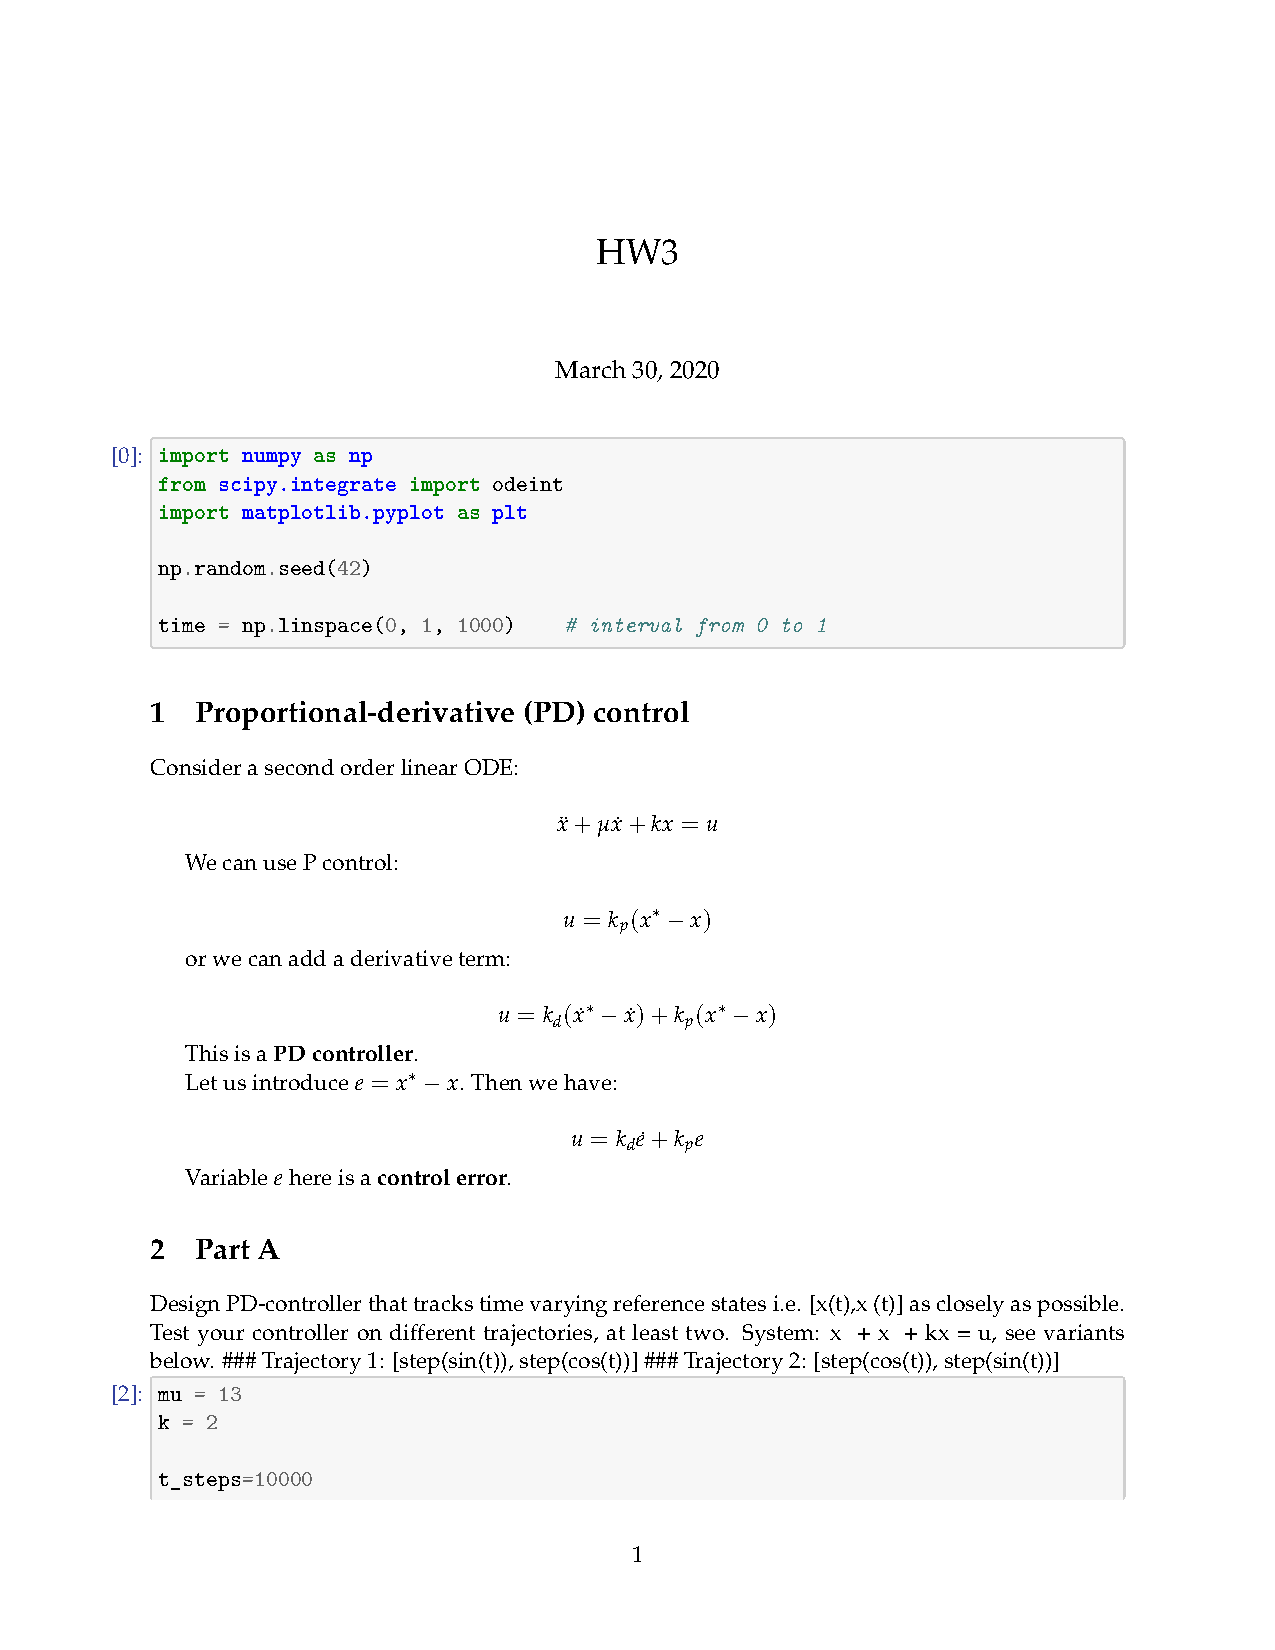
\includepdf[pages=-]{HW3_task1.pdf}


\section*{Problem 1}
Consider classical benchmark system in control theory - inverted pendulum on a cart (Figure 1). It is nonlinear under-actuated system that has the following dynamics.
  $$(M + m)\ddot{x} - ml \cos(\theta) \ddot{\theta}+ ml \sin(\theta) \dot{\theta}^2 = F$$
$$- \cos(\theta)\ddot{x} + l\ddot{\theta}- g \sin(\theta) = 0$$
\begin{center}
    where $g = 9.81$ is gravitational acceleration.
    $$(c)M = 15.1,m = 1.2,l = 0.35$$
    $$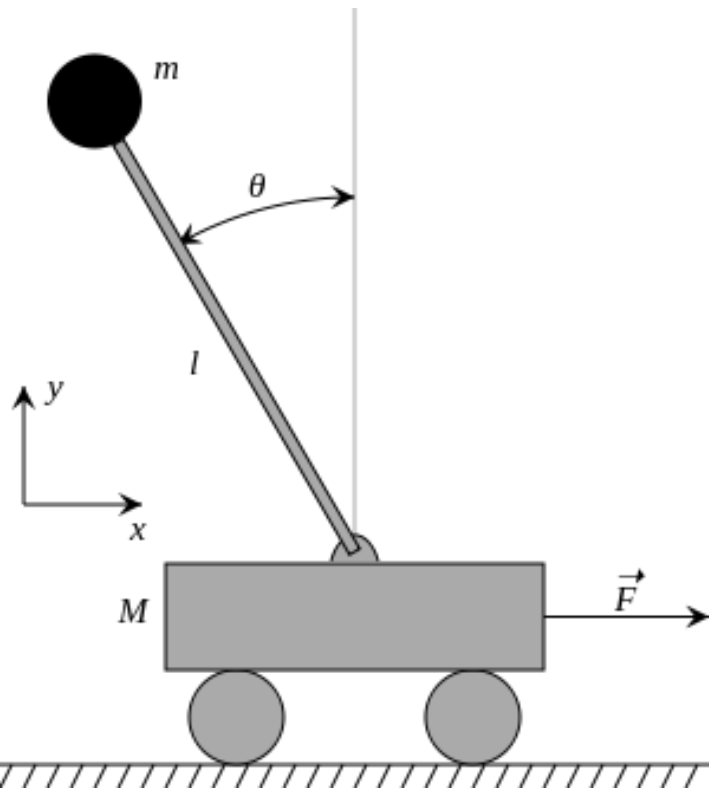
\includegraphics[width=10cm, height=10cm]{scheme.png}$$
    Figure 1: A schematic drawing of the inverted pendulum on a cart. The rod is considered massless. The mass of the cart and the point mass at the end of the rod are denoted by M and m. The rod has a length l.
\end{center}



\section*{part A}
\begin{problem}
  \problemquestion{Write equations of motion of the system in manipulator form 
$$M (q)\ddot{q} + n(q, \dot{q}) = Bu$$
    - where $u = F$, $q = \begin{bmatrix}x & \theta\end{bmatrix}^T$ is vector of generalized coordinates;}
  \problemsolution{$$\begin{bmatrix}M+m & -mlcos(\theta) \\  -cos(\theta) & l \end{bmatrix}\ddot{q} + \begin{bmatrix}ml sin(\theta) \dot{\theta}^2 \\ - gsin(\theta)  \end{bmatrix}= \begin{bmatrix} 1\\ 0\end{bmatrix}u$$
  
  $$Answer: \begin{bmatrix}16.3 & -0.42cos(\theta) \\  -cos(\theta) & 0.35 \end{bmatrix}\ddot{q} + \begin{bmatrix}0.42 sin(\theta) \dot{\theta}^2 \\ - gsin(\theta)  \end{bmatrix}= \begin{bmatrix} 1\\ 0\end{bmatrix}u$$
  }
\end{problem}


\section*{part B}
\begin{problem}
  \problemquestion{ Write dynamics of the system in control affine nonlinear form
$\dot{z} = f (z) + g(z)u$
    - where $z = \begin{bmatrix}x & \theta & \dot{x} & \dot{\theta}\end{bmatrix}^T$ is vector of states of the system;}
  \problemsolution{$\ddot{x}$:
$$\ddot{Q} = \frac{1}{l}(gsin(\theta) + cos(\theta)\ddot{x})$$
$$\Rightarrow (M+m(1-cos^2(\theta)))\ddot{x} - mgsin(\theta)cos(\theta)+mlsin(\theta)\dot{\theta}^2 = F$$
$$\ddot{x} = \frac{msin(\theta)(gcos(\theta)-l\dot{\theta}^2) + F}{(M+msin^2(\theta))}$$

$\ddot{\theta}$:
$$\ddot{x} = \frac{gsin(\theta) - l\ddot{\theta}}{-cos(\theta)}$$
$$\Rightarrow -g(M+m)tan(\theta)+\frac{l(M+m)}{cos(\theta)} \ddot{\theta} - mlcos(\theta)\ddot{\theta}+mlsin(\theta)\dot{\theta}^2 = F$$
$$\ddot{\theta}(l\frac{M + msin^2(\theta)}{cos(\theta)}) = g(M+m)tan(\theta)-mlsin(\theta)\dot{\theta}^2 + F$$
$$\ddot{\theta}=\frac{ g(M+m)sin(\theta)-mlsin(\theta)cos(\theta)\dot{\theta}^2 + cos(\theta)F}{l(M + msin^2(\theta))}$$

$\dot{z}$:
$$\dot{z}=\begin{bmatrix}\dot{x} \\ \dot{\theta} \\ \ddot{x} \\ \ddot{\theta} \end{bmatrix}=
\begin{bmatrix}
\dot{x}\\ 
\dot{\theta}\\ 
\frac{msin(\theta)(gcos(\theta)-l\dot{\theta}^2)}{(M+msin^2(\theta))} \\ 
\frac{ g(M+m)sin(\theta)-mlsin(\theta)cos(\theta)\dot{\theta}^2}{l(M + msin^2(\theta))}
\end{bmatrix}+ 
u\begin{bmatrix}0\\0\\ 
\frac{1}{(M+msin^2(\theta))} \\ \frac { 1}{l(M + msin^2(\theta))}\end{bmatrix}$$}
\end{problem}


\section*{part C}
\begin{problem}
  \problemquestion{Linearize nonlinear dynamics of the systems around equilibrium point $\bar{z} = \begin{bmatrix} 0 & 0 & 0 &0\end{bmatrix}^T$
$$\delta \dot{z} = A\delta z + B \delta u$$}
  \problemsolution{$$A =\frac{\delta f}{\delta z} = \begin{bmatrix} \frac{df}{dx} \\ \frac{df}{d\theta} \\ \frac{df}{\dot{dx}} \\ \frac{df}{d\dot{\theta}} \end{bmatrix} $$

$$f = \begin{bmatrix}
\dot{x}\\ 
\dot{\theta}\\ 
\frac{msin(\theta)(gcos(\theta)-l\dot{\theta}^2)}{(M+msin^2(\theta))} \\ 
\frac{ g(M+m)sin(\theta)-mlsin(\theta)cos(\theta)\dot{\theta}^2}{l(M + msin^2(\theta))}
\end{bmatrix} $$

$$\frac{df}{dx} = \begin{bmatrix} 0 & 0 & 0 & 0 \end{bmatrix}^T$$
$$\frac{df}{d\theta} = \begin{bmatrix} 0 & 0 & \frac{gm}{M} & \frac{g(M+m)}{lM} \end{bmatrix}^T$$
$$\frac{df}{d\dot{x} } = \begin{bmatrix} 1 & 0 & 0 & 0 \end{bmatrix}^T$$
$$\frac{df}{d\dot{\theta}} = \begin{bmatrix} 0 & 1 & 0 & 0 \end{bmatrix}^T$$

$$A = \frac{\delta f}{\delta z} = \begin{bmatrix} 0 & 0 & 0 & 0 \\ 0 & 0 & \frac{gm}{M} & \frac{g(M+m)}{lM}  \\ 1 & 0 & 0 & 0\\ 0 & 1 & 0 & 0 \end{bmatrix}^T=\begin{bmatrix} 0&0&1&0\\ 0&0&0&1 \\ 0&\frac{gm}{M}&0&0\\ 0&\frac{g(M+m)}{lM}&0&0\end{bmatrix}$$

$$B =\begin{bmatrix} 0 \\ 0 \\ \frac{1}{M} \\ \frac{1}{lM} \end{bmatrix}$$

$$Answer: A = \begin{bmatrix} 0&0&1&0\\ 0&0&0&1 \\ 0&0.7796&0&0\\ 0&30.256&0&0\end{bmatrix} $$
$$B =\begin{bmatrix} 0 \\ 0 \\ 0.066 \\ 0.189 \end{bmatrix}$$

}
\end{problem}


\section*{part D}
\begin{problem}
  \problemquestion{Check stability of the linearized system using any method you like;}
  \problemsolution{Find the eighen-values of A matrix:
$$det(\begin{bmatrix} -\lambda&0&1&0\\ 0&-\lambda&0&1 \\ 0&\frac{gm}{M}&-\lambda&0\\ 0&\frac{g(M+m)}{lM}&0&-\lambda\end{bmatrix}) = -\lambda(-\lambda^3 + \lambda\frac{g(M+m)}{lm}) = $$
$$\lambda^4-\lambda^2(\frac{gM+m}{lM}) = 0$$

$$\lambda = 0$$
$$\lambda = \sqrt{\frac{g(M+m)}{lM}} $$
$$\lambda = -\sqrt{\frac{g(M+m)}{lM}}$$


$$\lambda = \sqrt{\frac{9.81(16.3)}{5.285}} $$
$$\lambda = -\sqrt{\frac{9.81(16.3)}{5.285}}$$

$$\lambda = 5.5005461 $$
$$\lambda = -5.5005461 $$

$Answer:$ Thus there exist lambda with module that greater than zero => system without control is not stable}
\end{problem}


\section*{part E}
\begin{problem}
  \problemquestion{check if linearized system is controllable; if not - try another variant
or change values of your variant and find controllable.}
  \problemsolution{Sysem is controllable, when rank of matrix C is equal to 4, where $C =\begin{bmatrix}B & AB & A^2B &A^3B \end{bmatrix}$

$$A^2 = \begin{bmatrix} 0&\frac{gm}{M}&0&0 \\ 0&\frac{g(M+m)}{lM}&0&0 \\ 0&0&0&\frac{gm}{M} \\ 0&0&0&\frac{g(M+m)}{lM}\end{bmatrix}, A^2B= \begin{bmatrix}0\\0\\ \frac{gm}{M^2}\\ \frac{g(M+m)}{(lM)^2}\end{bmatrix}$$

$$A^3 = \begin{bmatrix} 0&0&0&\frac{gm}{M} \\ 0&0&0&\frac{g(M+m)}{lM} \\ 0&\frac{g^2m(M+m)}{lM^2}&0&0 \\ 0&(\frac{g(M+m)}{lM})^2&0&0\end{bmatrix}, A^3B = \begin{bmatrix}\frac{gm}{lM^2}\\ \frac{g(M+m)}{(lM)^2}\\0\\0\end{bmatrix}$$

$$
C = \begin{bmatrix} 
0&\frac{1}{M}&0&\frac{gm}{lM^2}\\ 
0&\frac{1}{lM}&0&\frac{g(M+m)}{l^2M^2}\\ 
\frac{1}{M}&0&\frac{gm}{M^2}&0\\ 
\frac{1}{lM}&0&\frac{g(M+m)}{l^2M^2}&0\end{bmatrix}$$

If ranc of C is less, then 4, then $\lambda= 0$ - one of its eig values, thus, the determinant of matrix C is zero itself. 

$$det(C) = -\frac{1}{M}(\frac{1}{M}(\frac{g(M+m)}{l^2M^2})^2-\frac{g^2m(M+m)}{(lM)^3M^2})-\frac{gm}{lM^2}(\frac{gm}{(lM)^2M^2}-\frac{g(M+m)}{M(lM)^3})=$$
$$ = \frac{g^2}{M^4l^2}(-(M+m)^2+m(M+m)-m^2+m(M+m))= \frac{g^2}{M^4l^2}((M+m)(-M+m)-m^2) = $$
$$ = \frac{g^2}{M^4l^2}(-M^2) = \frac{-g^2}{M^2l^2}\ne0$$

$Answer:$ all eig != 0 and rank(C) = 4 => system is controllable}
\end{problem}


\section*{part F}
\begin{problem}
  \problemquestion{(for the controllable system) design state feedback controller for lin- earized system using pole placement method. Assess the performance of the controller for variety of initial conditions. Justify the choice of initial conditions. Solve the task by two ways: using root-locus and with python. Compare them;}
  \problemsolution{Initial conditions were chosen such that system will converge with different speed to demonstrate how controller will act}
\end{problem}

Using root-locus method \\
\href{https://www.mathworks.com/help/control/ref/place.html}{Link to the Matlab method}
\begin{lstlisting}
>> g = 9.81;
M = 0.2;
m = 1;
l = 0.1;
>> A = [[0, 0, 1, 0]; [0, 0, 0, 1]; [0, g*m/M, 0, 0]; [0, g*(M+m)/l/M, 0, 0]];
B = [0; 0; 1/M; 1/l/M];
eig_vals = [-0.1 + 1j, -0.1 - 1j, -6 + 1j, -6 - 1j];
>> [K,prec,message] = place(A,B,eig_vals);
>> K

K =

   -0.0762   12.5878   -0.0398    0.2480

>> eig(A - B*K)

ans =

  -6.0000 + 1.0000i
  -6.0000 - 1.0000i
  -0.1000 + 1.0000i
  -0.1000 - 1.0000i
\end{lstlisting}

Using python
\begin{lstlisting}[label={list:first}]
import numpy as np
import matplotlib.pyplot as plt
import scipy.signal as sig
from scipy.integrate import odeint

g = 9.81
M = 0.2
m = 1
l = 0.1

eig_1 = [-0.25, -0.5, -1, -2]
eig_2 = [-1.1, -1.2, -1.3, -1.4]
eig_3 = [-0.1 + 1j, -0.1 - 1j, -6 + 1j, -6 - 1j]

A = np.array([[0, 0, 1, 0], [0, 0, 0, 1], [0, g*m/M, 0, 0], [0, g*(M+m)/l/M, 0, 0]])
B = np.array([0, 0, 1/M, 1/l/M]).reshape(-1, 1)
res_pole = sig.place_poles(A, B, eig_3)
K = res_pole.gain_matrix

# visualization
def control(x, t):
    return np.dot(A - np.dot(B, K), x)

time = np.linspace(0, 45, 1000)   
x0 = (np.random.random(4)) 
res = odeint(control, x0, time).T

fig = plt.figure(figsize=(8, 8))
plt.title("Stabilisation of the system")
plt.xlabel("time")
plt.plot(time, res[0], "r-", label="x")
plt.plot(time, res[1], "b-", label="$\theta$")
plt.plot(time, res[2], "k-", label="$\dot{x}$")
plt.plot(time, res[3], "g-", label="$\dot{\theta}$")
plt.grid()
plt.legend(shadow=True)
plt.show()
\end{lstlisting}

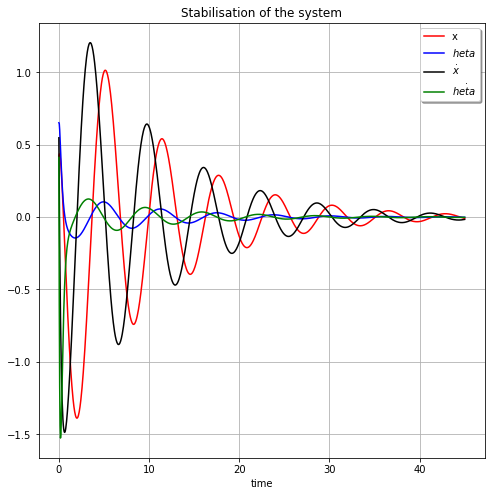
\includegraphics[width=10cm, height=10cm]{F.png}




\section*{part G}
\begin{problem}
  \problemquestion{(for the controllable system) design linear quadratic regulator for linearized system. Assess the performance of the controller for variety of initial conditions. Justify the choice of initial conditions;
  \problemsolution{Initial conditions were chosen such that system will behave differently}
}
\end{problem}

\begin{lstlisting}[label={list:second}]
import scipy.linalg as lin
#3
M = 0.2
m = 1
l = 0.1
#2
# M = 0.02
# m = 0.01
# l = 0.5

#1
# M = 0.01
# m = 0.001
# l = 0.1

# A, B - the same

A = np.array([[0, 0, 1, 0], [0, 0, 0, 1], [0, g*m/M, 0, 0], [0, g*(M+m)/l/M, 0, 0]])
B = np.array([0, 0, 1/M, 1/l/M]).reshape(-1, 1)

# Q, R - random, but appropriate
Q = np.array([[1, 0, 0, 0], 
              [0, 1, 0, 0], 
              [0, 0, 1, 0], 
              [0, 0, 0, 1]])
# R = np.array([-0.4]) #1
R = np.array([4]) #1

S = lin.solve_continuous_are(A, B, Q, R)

k = np.array(1/R[0]).dot(B.T).dot(S)

def simulator(x, t):
    return (A - np.dot(B, k)).dot(x)

time = np.linspace(0, 15, 1000)  
res = odeint(simulator, x0, time).T

fig = plt.figure(figsize=(8, 8))
plt.title("Stabilisation of the system")
plt.xlabel("time")
plt.plot(time, res[0], "r-", label="x")
plt.plot(time, res[1], "b-", label="$\theta$")
plt.plot(time, res[2], "k-", label="$\dot{x}$")
plt.plot(time, res[3], "g-", label="$\dot{\theta}$")
plt.grid()
plt.legend(shadow=True)
plt.show()

\end{lstlisting}

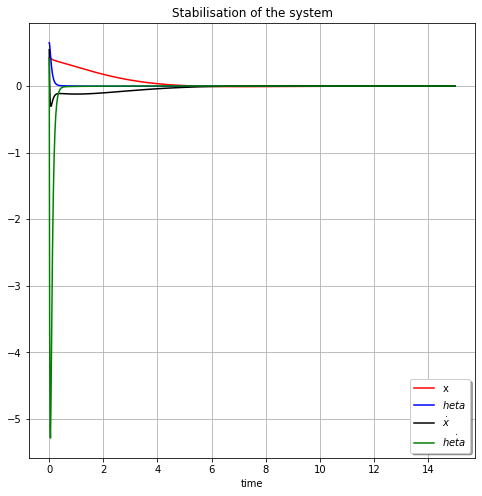
\includegraphics[width=10cm, height=10cm]{G.png}

\end{document}
